\documentclass{standalone}
\usepackage{graphicx}	
\usepackage{amssymb, amsmath}
\usepackage{color}

\usepackage{tikz}
\usetikzlibrary{calc, arrows.meta}
\usepackage{pgfmath}

\definecolor{light}{RGB}{220, 188, 188}
\definecolor{mid}{RGB}{185, 124, 124}
\definecolor{dark}{RGB}{143, 39, 39}
\definecolor{highlight}{RGB}{180, 31, 180}
\definecolor{gray10}{gray}{0.1}
\definecolor{gray20}{gray}{0.2}
\definecolor{gray30}{gray}{0.3}
\definecolor{gray40}{gray}{0.4}
\definecolor{gray60}{gray}{0.6}
\definecolor{gray70}{gray}{0.7}
\definecolor{gray80}{gray}{0.8}
\definecolor{gray90}{gray}{0.9}
\definecolor{gray95}{gray}{0.95}

\newcommand*{\offset}{0.025}

\begin{document}

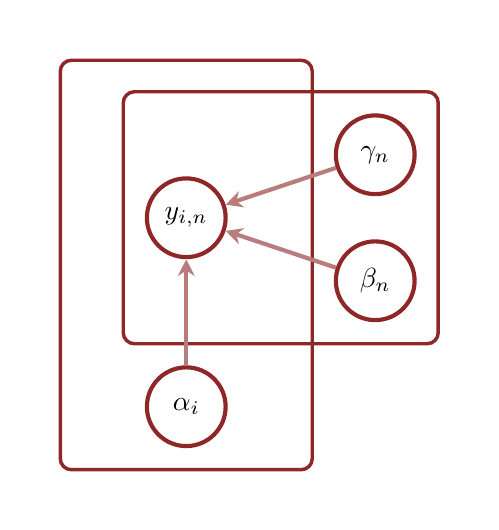
\begin{tikzpicture}[scale=0.2, thick]

  \pgfmathsetmacro{\r}{2.5}
    
  \draw[white] (-10, 14) rectangle (18, 44);

  \coordinate (A) at (0, 0);

  \coordinate (B) at (0, 8);
  
  \coordinate (C) at (-12, 2);
  \coordinate (D) at (-12, 8);
  \coordinate (E) at (-12, 14);
  
  \coordinate (F) at (0, 20);
  \coordinate (G) at (-12, 20);
  
  \coordinate (H) at (12, 28);
  \coordinate (I) at (12, 36);
  
  \coordinate (J) at (0, 32);
  
  \draw[dark, line width=1.25, rounded corners=4] (-8, 16) rectangle (8, 42);
  \draw[dark, line width=1.25, rounded corners=4] (-4, 24) rectangle (16, 40);

  \foreach \B/\E in {F/J, H/J, I/J} {
    \draw[-{Stealth[length=6pt, width=6pt]}, shorten <=15, shorten >=15, color=mid, line width=1.5] (\B) -- (\E);
  }
  
  \filldraw[fill=white, draw=dark, line width=1.5] (F) circle (\r)
  node[color=black] { $\alpha_{i}$ };
  
  \filldraw[fill=white, draw=dark, line width=1.5] (H) circle (\r)
  node[color=black] { $\beta_{n}$ };
  
  \filldraw[fill=white, draw=dark, line width=1.5] (I) circle (\r)
  node[color=black] { $\gamma_{n}$ };
  
  \filldraw[fill=white, draw=dark, line width=1.5] (J) circle (\r)
  node[color=black] { $y_{i, n}$ };

\end{tikzpicture}

\end{document}  